\chapter[Declarative Rewrite: Magic-sets]{Declarative Rewrite: Magic-sets}
\label{ch:magic}

Having described the Evita Raced infrastructure, we now turn to our use of it
to specify query optimizations in \OVERLOG.  Using Evita Raced, we have
implemented three optimization techniques from the literature: the magic-sets
rewrite~\cite{magic-sets1, magic-sets2}, the System R dynamic
program~\cite{selinger} and the Cascades branch-and-bound
algorithm~\cite{cascades}.  We begin in this chapter with the magic-sets
rewrite, which aims to efficiently answer predicates pertaining to a small
subset of the data values in the database.  For example, the \ol{shortestPath}
predicate in Figure~\ref{ch:p2:fig:overlogSP} pertains to paths originating
from node ``localhost:10000.'' In order to efficiently evaluate this predicate,
the magic-sets rewrite pushes predicate constants down into the supporting
rules so that a Datalog evaluator {\em never} derives superfluous facts.

As mentioned in Chapter~\ref{ch:p2:sec:eval}, Datalog-oriented systems like P2
perform a bottom-up ({\em forward chaining}) evaluation on each rule, starting
with known facts (tuples), and recursively deriving new facts through rule
deductions.  The advantage of this strategy is that the evaluation is data
driven (from known facts to possible deductions) and will not enter infinite
loops for some statically verifiable {\em safe} programs.  In contrast, a
top-down ({\em backward chaining}) evaluation (e.g., in the Prolog language),
starts with the ``query'' predicates (i.e., \ol{shortestPath}
in Figure~\ref{ch:p2:fig:overlogSP}) as the top-level goals, and recursively
identifies rules whose head predicates unify with needed goals, replacing them
with the subgoal predicates in the rule body, until all subgoals are satisfied
by known facts or rejected when no further recursion is possible.  The
advantage of a top-down evaluation strategy is that it avoids resolving goals
that are not needed by the posed queries (e.g., paths not originating from
``localhost:10000'').

For a given Datalog program, the magic-sets rewrite adds extra rules and
predicates that prune results, known to be superfluous, from a bottom-up
evaluation.  The primary data structure used by this rewrite technique is a
rule/goal graph, which we review in Chapter~\ref{ch:magic:sec:review}, along
with the magic-sets algorithm.  Using the rule/goal graph representation of an
\OVERLOG program, in Chapter~\ref{ch:magic:sec:rules} we express the magic-sets
rewrite in $44$ \OVERLOG rules.  We divide these rules into two logical groups.
The first is presented in Chapter~\ref{ch:magic:sec:rgconstruct}, which
constructs the rule/goal graph via a transitive closure on the Metacompiler
Catalog.  Our second group of rules, presented in
Chapter~\ref{ch:magic:sec:rewrite}, also performs a transitive closure, but
this time on the rule/goal graph itself, to obtain the rewritten rules that
include the predicates used to filter tuples that are not relevant to the final
answer.

\section{Magic-sets in a Nutshell}
\label{ch:magic:sec:review}

\begin{figure*}[!t]
\ssp
\centering
\begin{lstlisting}
link(``node1'', ``node2'', 1).
link(``node1'', ``node3'', 1).
link(``node2'', ``node1'', 1).
...
r1 path(@X, Y, P, C) :-
   link(@X, Y, C), P := f_cons(X, Y).

r2 path(@X, Z, P, C) :-
   link(@X, Y, C1), path(@Y, Z, P2, C2),
   f_contains(X, P2) == false,
   P := f_cons(X, P2), C := C1 + C2.

query path(``node1'', Y, P, C).
\end{lstlisting}
\caption{\label{ch:magic:fig:basicSP}The path-only rules copied from Figure~\ref{ch:p2:fig:overlogSP}.}
\end{figure*}

\begin{figure*}
\centering
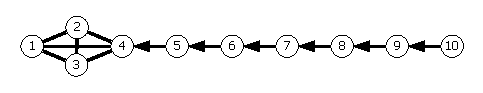
\includegraphics[scale=1.2]{figures/Topology}
\caption{Experimental topology.}
\label{ch:magic:fig:topo}
\end{figure*}

The magic-sets technique rewrites logical rules so that bottom-up evaluation
over the rewritten rules has all the advantages of a top-down and a bottom-up
evaluation strategy.  We give some intuition here by reviewing the advantages
of magic-sets using the path program shown in
Figure~\ref{ch:magic:fig:basicSP}.  For the purpose of this discussion, lets
assume we execute these rules locally with the initial set of \ol{link} fact
tuples forming the topology shown in Figure~\ref{ch:magic:fig:topo}.  The
abbreviated list of facts shown at the beginning of
Figure~\ref{ch:magic:fig:basicSP} populate the \ol{link} relation with our
basic topology information.  Our goal is to find all paths that start at
``node1.''

A straightforward bottom-up evaluation of this program applies the \ol{link}
tuples to rule \ol{r1}, creating the initial set of {\tt path} tuples.  Rule
\ol{r2} performs a transitive closure over the \ol{link} and \ol{path}
relations, while any \ol{path} tuples matching ``node1'' in the first field are
returned in the programmer's query.  Clearly this bottom-up evaluation strategy
examines some \ol{path} tuples that do not contribute to the query answer; for
example, paths that originate from nodes $5-10$~\footnote{Paths that originate
from nodes~$2-4$ are still relevant since they can be included in paths
originating from ``node1.''}.  In contrast, a top-down evaluation begins by
unifying the query predicate with the head predicate of rules \ol{r1} and
\ol{r2}.  This \ol{path} predicate unification binds the $@X$ attribute to
``node1'' in both rules, which is then carried over to the predicates in the
rule body.

The magic-sets rewrite is an optimization that can achieve the same
efficiency found in the top-down evaluation, using a bottom-up evaluator.
Since it is still bottom-up, we retain all the benefits of semina\"{\i}ve
evaluation: set-oriented evaluations, unique minimal model and stratification.
Magic-sets does this by adding extra selection predicates to the rules of a
program that emulate the goal-oriented execution of a top-down evaluation
(sometimes called {\em sideways information passing} or SIP).  Conceptually,
given a rule of the form $H\ \text{\ol{:-}}\ G_1, G_2, ..., G_k$, where $H$ is
the head predicate and $G_{1,...,k}$ are the subgoals, the magic-sets rewrite
intersperses selection predicates $s_{1,...,k}$ to generate the rule form $H\
\text{\ol{:-}}\ s_1, G_1, s_2, G_2, ..., s_{k}, G_k$.  Facts for these
selection predicates are generated according to attribute bindings in the
user's query or from other rule predicates in the program, to constant values.

\begin{figure*}[!t]
\ssp
\begin{lstlisting}
link(``node1'', ``node2'', 1).
link(``node1'', ``node3'', 1).
link(``node2'', ``node1'', 1).
...
magic_path(``node1'').

r1_case5 path(@X, Y, P, C) :-
         magic_path(@X),
         link(@X, Y, C), P := f_cons(X, Y).

r2_case2 sup_r2_1(@X, Y, C1) :-
         magic_path(@X),
         link(@X, Y, C1).

r2_case3 magic_path(@Y) :-
         sup_r2_1(@X, Y, C1).

r2_case4 sup_r2_2(@X, Y, Z, C1, P2, C2) :-
         sup_r2_1(@X, Y, C1),
         path(@Y, Z, P2, C2).

r2_case5 path(@X, Z, P, C) :-
         sup_r2_2(@X, Y, Z, C1, P2, C2),
         f_contains(X, P2) == false,
         P := f_cons(X, P2), C := C1 + C2.

query path(``node1'', Y, P, C).
\end{lstlisting}
\caption{\label{ch:magic:fig:magicSP}A magic-sets rewrite of 
the rules in Figure~\ref{ch:magic:fig:basicSP}.}
\end{figure*}

Figure~\ref{ch:magic:fig:magicSP} shows the rewritten rules from the path
program in Figure~\ref{ch:magic:fig:basicSP}.  The program contains some new
predicates prefixed with \ol{magic\_} and \ol{sup\_} that are included in the
rule body with the \ol{link} and \ol{path} predicates.
Ullman~\cite{ullmanbook} refers to these new predicates as magic predicates
(i.e., \ol{magic\_path}) and supplementary predicates (i.e., \ol{sup\_r2\_1},
\ol{sup\_r2\_2}).  Magic predicates maintain bindings relevant to query
predicates (i.e., \ol{path}), while supplementary predicates pass bindings
along rule bodies, ensuring that no extraneous deductions are made along the
way.

We now describe the rewritten rules, which are named by 1) the original rule
name, and 2) a ``case'' number that will be described in
Chapter~\ref{ch:magic:sec:rewrite}.~\footnote{Case 1 refers to the creation of
the single magic predicate \ol{magic\_path} fact, which contains the bound
constants from the query predicate.} We start with rule~\ol{r1} in
Figure~\ref{ch:magic:fig:basicSP}, again assuming we are running locally with
all facts in the \ol{link} relation.  As it stands, rule~\ol{r1} will generate
\ol{path} tuples using any of the \ol{link} tuples, regardless of whether they
contribute to answering the final query.  To avoid extraneous deductions, we
add the \ol{magic\_path} predicate to the body of this rule, giving us
rule~\ol{r1\_case5} in Figure~\ref{ch:magic:fig:magicSP}.

The rewrite of rule~\ol{r2} appears to be quite a bit more complicated,
expanding out to four separate rules.  We describe the purpose of each rule on
a case-by-case basis.  Rule~\ol{r2\_case2} adds a rule that fills the
\ol{sup\_r2\_1} relation with tuples produced by ``joining'' \ol{magic\_path}
and \ol{link} relations.  The outcome of which is no different than
rule~\ol{r1\_case5} in our previous discussion; excluding the extra path
information.  The interesting bit here is that, in rule~\ol{r2\_case4}, the
\ol{sup\_r2\_1} predicate is ``joined'' with the \ol{path} predicate.  This
effectively uses the \ol{magic\_path} predicate to prune superfluous tuples
from \ol{link} before ``joining'' with the \ol{path} relation.

This brings us to the more interesting case~$3$ w.r.t.\@ rule~\ol{r2}.  Here we
are feeding \ol{sup\_r2\_1} tuples into the \ol{magic\_path} relation.  At a
high-level, this rule updates the \ol{magic\_path} table with tuples that
satisfy the constraints imposed by the current \ol{magic\_path} table instance
and includes the new (path) information from the \ol{link} predicate.  Observe
that rule~\ol{r2\_case3} feeds \ol{magic\_path} values from its $Y$ variable,
which represents the intermediate hop in rule~\ol{r2}, and therefore must be
part of the final answer.  In this example, rule~\ol{r2\_case3} is responsible
for adding each node in the clique (i.e., nodes 2, 3, and 4 in
Figure~\ref{ch:magic:fig:topo}) to the \ol{magic\_path} relation because there
is a path from ``node1'' to it.

The remaining cases simply stitch things up using the remaining terms in
rule~\ol{r2}.  In case~$4$, we combine \ol{sup\_r2\_1} with the \ol{path}
predicate to obtain the \ol{sup\_r2\_2}, which is then used to finish off the
rule in case~$5$ (rule~\ol{r2\_case5}).  The reader may be confused by the need
for \ol{sup\_r2\_2}. Why not simply create the following rule? 
\begin{lstlisting}
r2_case? path(@X, Z, P, C) :-
         sup_r2_1(@X, Y, C1),
         path(@Y, Z, P2, C2).
         f_contains(X, P2) == false,
         P := f_cons(X, P2), C := C1 + C2.
\end{lstlisting}
Indeed, this rule is correct and it does not generate paths that are not relevant to
the final answer.  Nevertheless, we introduce the \ol{sup\_r2\_2} predicate
(case~$4$), in general, since we do not know if this is the last occurrence of
a magic predicate (i.e., \ol{path}) in rule~\ol{r2}.  The occurence of a magic
predicate~$p$ in rule~$r$ at position~$j$ triggers cases $2$ and $3$, which
generate rules in the following form.
\begin{itemize}
  \item case 2: $sup^r_j(...) \ol{:-} sup^r_{i-1}(...), G_i, ..., G_{j-1}$
  \item case 3: $magic_p(...) \ol{:-} sup^r_j(...)$
\end{itemize}
The subgoals $G_{i...j-1}$ refer to EDB predicates appearing in the body of
rule~$r$ at the respective positions.  Returning to our example, case $4$
anticipates the need for generating a \ol{sup\_r2\_X} predicate, which will use
\ol{sup\_r2\_2} and all subseqent EDB predicates to generate case $2$.
Furthermore, case~$3$ requires \ol{sup\_r2\_X} to update the magic (IDB)
predicate appearing in rule~\ol{r2} at position~\ol{X}.  In keeping with the
current numbering scheme, we note that $\ol{sup\_r2\_0 :- magic\_path}$.

Before presenting the declarative rules that implement this rewrite technique,
we must review the concept of adornments and the rule/goal graph representation
for a collection of Datalog (\OVERLOG) rules.  These data structures form the
basis of the transitive closure algorithm performed by our magic-sets rewrite.
The discussion leading up to Chapter~\ref{ch:magic:sec:rules} follows from
Chapter~$13$ of Ullman's textbook~\cite{ullmanbook}, which provides the most
through coverage on the subject to date.


\subsection{Adornments}

Consider again the path program in Figure~\ref{ch:magic:fig:basicSP}.  The
query predicate \ol{path(``node1'', Y, P, C)} asks for all paths that originate
from ``node1''.  An {\em adornment} is a binding pattern that contains a string
of {\em b's} (bound) and {\em f's} (free) of length {\em k}, for each {\em k}
arguments of \ol{path}.  In the current context, the {\em path} query predicate
matches the $path^{bfff}$ {\em adornment} since the first argument is bound to
a constant and the last three variables are free to take on any value.  Such
{\em goal adornments} are assigned to rule predicates, based on the position of
the predicate in the rule and the bindings associated with that rule position.

Rule bindings are assigned by position, according to a left-to-right (SIP)
evaluation order.  The steps for assigning {\em rule adornments} are as
follows.
\begin{enumerate}
    \ssp
    \item A variable appearing in a bound argument of the rule head is bound 
      before processing any subgoals i.e., $path^{bfff}$ binds $@X$ in the 
      \ol{path} head of rule~\ol{r2}.
    \item A variable is bound after processing subgoal $G_i$ if it was bound 
          before processing $G_i$ or if it appears anywhere in $G_i$ i.e.,
	  the \ol{link} subgoal binds the $@Y$ variable in the \ol{path} subgoal
	  of rule~\ol{r2} (variables $Z$, $P2$, and $C2$ in \ol{path} remain free).
\end{enumerate}
The format of a rule adornment differs from that of a predicate.  It follows the form
$[B_1,\cdots,B_m|F_1,\cdots,F_n]$, which contains two sublists of variables
separated by a bar.  The variables to the left of the bar (i.e.,
$B_1,\cdots,B_m$) represent bound variables, while those to the right (i.e.,
$F_1,\cdots,F_n$) are free. 

A given rule contains a number of these binding patterns, one for each subgoal
position.  That is, a rule adornment is a binding pattern of a rule at a given
rule position.  The notation that we follow here identifies the rule's position
as a subscript and the binding pattern as a superscript.  For example,
$r1_0^{[@X|Y,P,C]}$ is the adornment for rule \ol{r1} at position $0$, which is
based on the binding pattern of the $path^{bfff}$ adornment relative to the
head predicate schema.

Continuing, $r2_0^{[@X,|Y,Z,C1,P,C]}$ represents the adornment for rule~\ol{r2}
at the head position $0$, again binding the first variable of the head
predicate.  The $r1_0$ and $r2_0$ rule adornments ``feed'' the \ol{link}
subgoal with its bindings, create the $link^{bff}$ goal adornment.  The
\ol{link} subgoal adds variables $Y$ and $C1$ to the list of bound variables
for rule~\ol{r2} at position $1$.  This yields the $r2_1^{[@X,Y,C1,|Z,P,C]}$
rule adornment, which ``feed'' bindings into the \ol{path} predicate, creating
the $path^{bfff}$ adornment by binding the $Y$ variable in the first argument.

\subsection{Rule/Goal Graphs}

\begin{figure*}[!t]
\begin{center}
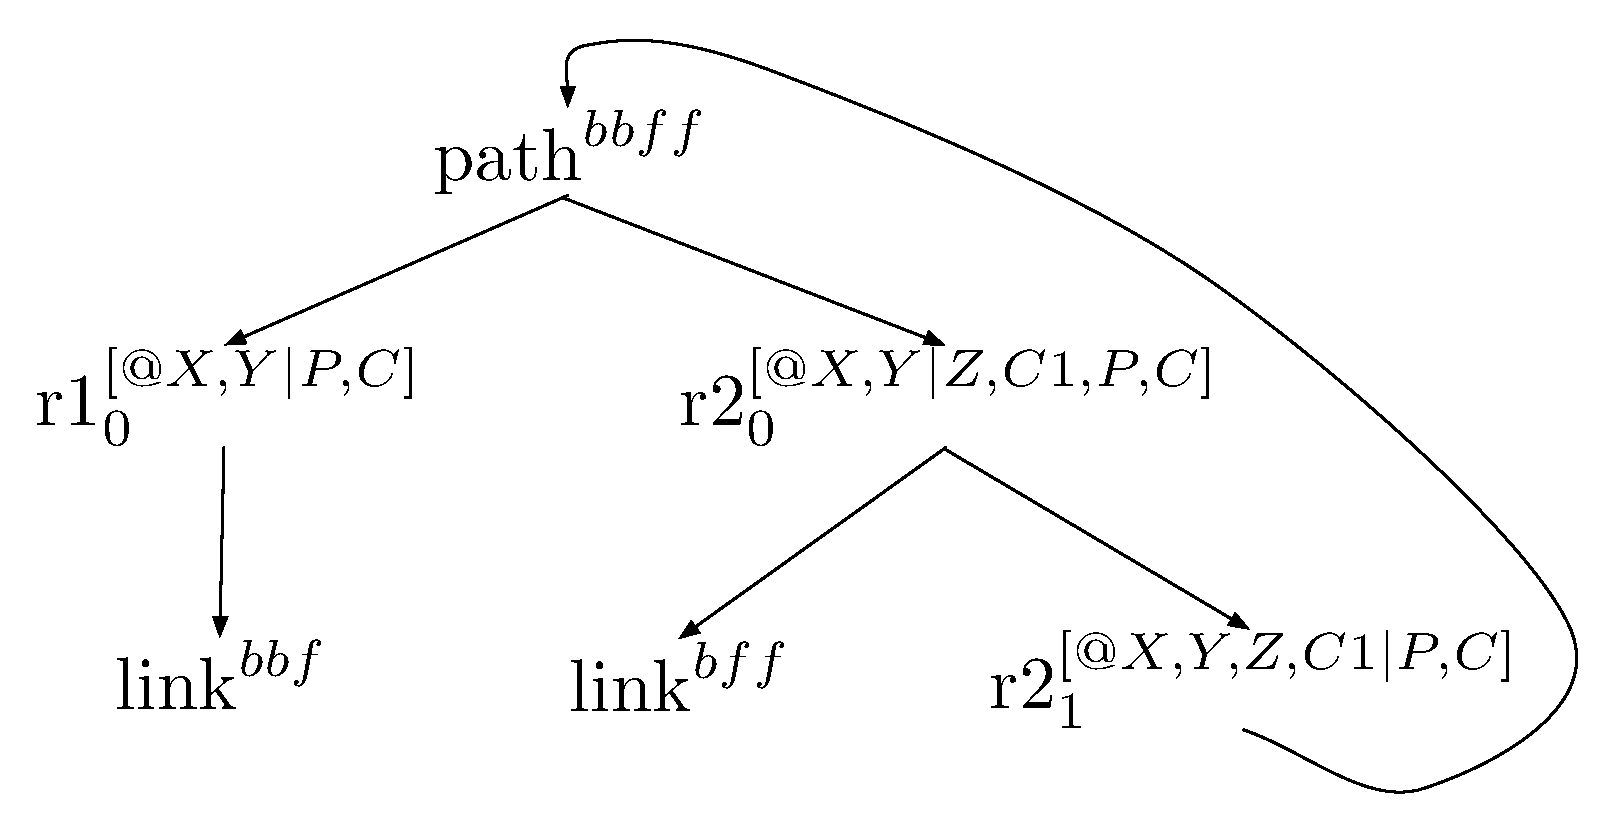
\includegraphics[scale=0.5]{figures/RuleGoalGraph}
\caption{\label{ch:magic:fig:rggraph}Rule/Goal graph of the program in Figure~\ref{ch:magic:fig:basicSP}.}
\end{center}
\end{figure*}

A rule/goal graph is a representation of binding patterns that occur in a
collection of Datalog (\OVERLOG) rules.  The graph consists of {\em rule} and
{\em goal} vertices.  A goal vertex consists of a predicate with an adornment
(e.g., $path^{bfff}$) and similarly, a rule vertex represents the adornment of
the rule in a particular position (i.e., $r1_0^{[@X|Y,P,C]}$).

Figure~\ref{ch:magic:fig:rggraph} illustrates the {\em rule/goal} graph for our
Figure~\ref{ch:magic:fig:basicSP} example.  To construct this graph, we start
at the query predicate, and create a goal vertex in the graph with its proper
adornment.  For every rule with that goal predicate as its head, we create a
rule adornment relative to position~$0$.  For rule~\ol{r1} this is
$r1_0^{[@X|Y,P,C]}$ and for rule~\ol{r2} we have $r2_0^{[@X,|Y,Z,C1,P,C]}$.  A
rule vertex feeds bindings to the subgoal just beyond its position.  Both rules
in position $0$ bind the \ol{link} predicate variable $X$.  In the case of
rule~\ol{r2}, position~$1$ receives the bindings of its parent rule and
the bindings from the \ol{link} subgoal, giving us the
$r1_1^{[@X,Y,C1,|Z,P,C]}$ rule vertex.

At this point in rule~\ol{r2} we have reached the position prior to the
\ol{path} predicate.  We create the appropriate $path^{bfff}$ adornment, which
matches up with our original \ol{path} goal node.  Since we have no further
rule binding steps beyond the path predicate, the process halts.  Our
declarative rules initiate the rewrite process by performing these steps
recursively over the Metacompiler Catalog.

\section{Declarative Magic-sets}
\label{ch:magic:sec:rules}

Using Evita Raced, we expressed the magic-sets rewrite stage in \OVERLOG.  The
first step in this rewrite constructs the rule/goal graph, captured as
relational data.  It uses this graph data to check for a {\em unique binding
property} with respect to the adornment of the query predicate.  This property
is met when the query predicate $q_p$, expressed against predicate $p$,
contains a unique ``binding pattern'' throughout the rule/goal graph.  The
query predicate $q_p$ provides the first binding pattern (the root of the
rule/goal graph), while rules that mention $p$ provide further bindings based
on sideways-information-passing (SIP).

We check for the unique binding property in the first phase of our rewrite,
while constructing the rule/goal graph via a transitive closure on the
Metacompiler Catalog.  If this property is violated at any point then the
rewrite terminates early, without changing any rules.  The Metacompiler Catalog
already provides some of the rule/goal graph information, specifically goal
(head predicate) and subgoal (body terms) rule dependencies.  The remaining
information that we need to collect is the adornments for rule/goal
``vertices.''  Once this information is secured, we can move to the actual
rewrite rules described in Chapter~\ref{ch:magic:sec:rewrite}, where magic and
supplementary relations are created according to the five cases previously
discussed.

\subsection{Rule/Goal Graph Construction}
\label{ch:magic:sec:rgconstruct}

The algorithm for constructing a rule/goal graph begins at the query predicate,
and follows with the rules that mention the query predicate in the head.  We
assume the unique binding property holds in the beginning, and detect if it
does not along the way.  Given a query predicate $q_p$, we create a {\em magic
predicate}, denoted as $m_p$, with a corresponding adornment.  A set of {\em
supplementary predicates}, denoted as $sup_i$ ($i$ being the rule position),
are also created as we recursively walk the rules in a left-to-right (SIP)
order.


\begin{figure*}[!t]
\ssp
\centering
\begin{lstlisting}
%* /* Create an adornment for the query predicate and add a fact to the \ol{magicPred}  \\
      table referencing this adornment. */ *)
ms1 magicPred(@A, Pid, Name, Sig) :-
    magic::programEvent(@A, Pid, ...),
    sys::rule(@A, Rid, Pid, ... , Goals),
    sys::predicate(@A, _, Rid, ..., Schema),
    Goals == 1,
    Sig := f_adornment(Schema).
\end{lstlisting}
\caption{\label{ch:magic:fig:magic1}Construction of the query adornment and corresponding magic predicate.}
\end{figure*}

The abbreviated rule in Figure~\ref{ch:magic:fig:magic1} creates an adornment
for the query predicate and adds that fact to the \ol{magicPred} relation.  A
query predicate is identified in P2 by a rule containing a single goal ($Goals
== 1$).  The sole predicate in this rule has a schema ($Schema$) that contains
some number of (binding) constants and (free) variables.  The function \ol{f\_adornment} 
takes such a schema object as its argument and returns a string
representing an adornment signature (the binding pattern).

Rule~\ol{ms1} creates the top-level goal node that represents the root of the
rule/goal graph.  The group of rules in Figure~\ref{ch:magic:fig:magic2} deal
with creating adornments for rule positions in the target program.  We store
the rule adornment in a \ol{sup} relation since this information will be used
to create supplementary predicates in Chapter~\ref{ch:magic:sec:rewrite}.  A
\ol{sup} tuple contains the following attributes in order:
\begin{itemize}
   \ssp
  \item A reference to the target program and rule identifiers. 
  \item A position within that target rule.
  \item A name for the supplementary predicate.
  \item A rule adornment, as a schema object containing all constants and variables up to that rule position.
  \item A new identifier that will be used (in Chapter~\ref{ch:magic:sec:rewrite}) to create 
    a new rule that supplies facts to the supplementary relation (e.g., rule cases $2$ and $4$ 
    in Figure~\ref{ch:magic:fig:magicSP}).
\end{itemize}

\begin{figure*}[!t]
\ssp
\centering
\begin{lstlisting}
%* /* Initialize sup position 0 for rules that reference a magic predicate in the head. */ *)
ms2 sup(@A, Pid, Rid, Pos, SupName, Schema, f_idgen()) :-
    magicPred(@A, Pid, Name, Sig),
    sys::rule(@A, Rid, Pid, RName, HeadPid, ...),
    sys::predicate(@A, HeadPid, Rid, _, Name, ..., FSchema, ...),
    Schema := f_project(Sig, FSchema),
    SupName := "sup_" + RName + 0,
    Pos := 0.

%* /* Create supplementary predicate for a given subgoal. */ *)
ms3 sup(@A, Pid, Rid, Pos, SupName, NewSchema, f_idgen()) :-
    supNext(@A, Pid, Rid, Pos, Schema),
    sys::rule(@A, Rid, Pid, RName, ...),
    sys::predicate(@A, Fid, Rid, ..., FSchema, Pos, ...),
    SupName := "sup_" + RName + "_" + Pos,
    NewSchema := f_merge(Schema, FSchema).
	
%* /* Create supplementary predicate for a given assignment. */ *)
ms4 sup(@A, Pid, Rid, Pos, SupName, NewSchema, f_idgen()) :-
    supNext(@A, Pid, Rid, Pos, Schema), 
    sys::rule(@A, Rid, Pid, RName, ...),
    sys::assign(@A, Aid, Rid, Var, _, Pos),
    SupName := "sup_" + RName + "_" + Pos,
    NewSchema := f_assignschema(Schema, Var).

%* /* Move the rule position forward when update occurs to sup. */ *)
ms5 supNext(@A, Pid, Rid, Pos+1, Schema) :-
    sup(@A, Pid, Rid, Pos, Name, Schema, Tid).
	
%* /* Move supNext forward for selection predicates. */ *)
ms6 supNext(@A, Pid, Rid, Pos+1, Schema) :-
    supNext(@A, Pid, Rid, Pos, Schema),
    sys::rule(@A, Rid, Pid, ..., Goals),
    sys::select(@A, Sid, Rid, _, Pos, _),
    Pos < Goals. 
\end{lstlisting}
\caption{\label{ch:magic:fig:magic2}Rules for supplementary relational predicates.}
\end{figure*}

We now describe the details of each rule in Figure~\ref{ch:magic:fig:magic2}.
Rule~\ol{ms2} initiates the first \ol{sup} deduction.  It joins \ol{magicPred}
with the \ol{rule} and \ol{predicate} relations to obtain those rules that
reference a magic predicate in the head.  This result will represent the
supplementary predicate in position~$0$.  The adornment for this rule position
is obtained by projecting the head predicate schema onto the magic predicate
adornment.  The function \ol{f\_project} takes care of the step-by-step
details of combining the head predicate schema and the signature of the magic
predicate adornment, and then returning a new schema that contains only the bound
head variables (according to the adornment).  For example, if the head
predicate schema is $[@X, Y, P, C]$ and the adornment is $bfff$ then the \ol{f\_project} 
will return $[@X]$ as the new schema.  The new schema is used by
the current (position~$0$) supplementary predicate.~\footnote{The supplementary
predicate at position~$0$ is a symbolic reference to the magic predicate.}

The rules that receive a \ol{sup} tuple are consider next by creating further
\ol{sup} tuples for each subgoal position.  In \OVERLOG, only table predicates
and ``assignment'' statements create new bindings.  As a result, \ol{sup}
tuples are only generated for rule positions relevant to such terms: relational
predicates (rule~\ol{ms3}) and assignment statements (rule~\ol{ms4}).  The
\ol{f\_merge} and \ol{f\_assignschema} functions are used to update the schema
object with the bindings of the current term position.  A series of
\ol{supNext} tuples is created for each rule position to considered.  The
\ol{supNext} relation is generated by rule~\ol{ms5} for predicate and
assignment terms, and rule~\ol{ms6} for selection predicate terms, which add no
new bindings to the previous schema.


\begin{figure*}[!t]
\ssp
\centering
\begin{lstlisting}
%* /* We've encountered a magic predicate in the body of a rule.  Compute its adornment based on \\
      current bound variables. */ *)
ms7 magicPred(@A, Pid, FName, Sig) :-
    supNext(@A, Pid, Rid, Pos, Schema),
    sys::rule(@A, Rid, Pid, RName, ...),
    sys::predicate(@A, Fid, Rid, _, FName, ..., FSchema, Pos, ...),
    magicPred(@A, Pid, FName, Sig),
    Sig := f_adornment(Schema, FSchema).
\end{lstlisting}
\caption{\label{ch:magic:fig:magic3}Encountering a magic predicate during subgoal traversal.}
\end{figure*}

The previous group of rules ignored the special case of discovering a magic
predicate at rule positions referenced by some \ol{supNext} tuples.  In order
to verify that the unique binding property holds, we must compute the adornment
for each magic predicate appearance in the rule body.
Figure~\ref{ch:magic:fig:magic3} contains the single rule that generates an
adornment for a subgoal that references a magic predicate.  If the adornment is
different than the previous, then multiple rows will exist in the
\ol{magicPred} relation, signaling the presence of multiple magic predicate
binding patterns.  A simple count query (Figure~\ref{ch:magic:fig:magic4}:
count~\ol{ms12} and check~\ol{ms13}) is used to detect violations of the unique
binding property.

\begin{figure*}[!t]
\ssp
\centering
\begin{lstlisting}
%* /* Indicate when a rule has been fully explored. */ *)
ms9 ruleComplete(@A, Pid, Rid) :-
    supNext(@A, Pid, Rid, Pos, _),
    sys::rule(@A, Rid, Pid, ..., Goals),
    Pos == Goals. 
	       
%* /* Count the number of completed rules. */ *)
ms10 rulesComplete(@A, Pid, a_count<Rid>) :-
     ruleComplete(@A, Pid, Rid).
	        
%* /* Count the number of rules in a program. */ *)
ms11 programRuleCount(@A, Pid, a_count<Rid>) :-
     programEvent(@A, Pid, ...),
     sys::rule(@A, Rid, Pid, ...).
	
%* /* Count the number of adornments for a given magic predicate. */ *)
ms12 countAdornments(@A, Pid, Name, a_count<Sig>) :-
     magicPred(@A, Pid, Name, Sig).
	       
%* /* Commit a magic predicate iff it has a unique adornment. */ *)
ms13 commitMagicPred(@A, Pid, Name, Sig, f_idgen()) :-
     programRuleCount(@A, Pid, RuleCount),
     rulesComplete(@A, Pid, RuleCount),
     countAdornments(@A, Pid, Name, Count),
     magicPred(@A, Pid, Name, Sig),
     Count == 1.
\end{lstlisting}
\caption{\label{ch:magic:fig:magic4}Detect completion of rule/goal traversal 
and check for unique binding property.}
\end{figure*}

The last group of rules detect when the rule/goal graph construction ``phase''
has completed, and on completion, checks for the unique binding property.  In
Figure~\ref{ch:magic:fig:magic4}, rules~\ol{ms9} and \ol{ms10} together count
the number of rules that have completed the rule/goal graph construction phase.
Rule~\ol{ms11} counts the total number of rules in a given program and
rule~\ol{ms12} counts the number of adornments for a given \ol{magicPred}.
Finally, rule~\ol{ms13} signals the completion of the current phase by deriving
a \ol{commitMagicPred} tuple if all rules have completed and the magic
predicate has a single adornment.  We note here that the counts for
\ol{programRuleCount} and \ol{rulesComplete} would not be needed if P2 had
support stratified Datalog.  The magic predicate adornment count is needed
before moving to the next phase, but it also marks a stratification boundary.
To prevent a premature \ol{commitMagicPred} deduction in rule~\ol{ms13}, we
ensure the counts in \ol{programRuleCount} and \ol{rulesComplete} are equal.


\subsection{Rewrite Phase}
\label{ch:magic:sec:rewrite}
 
At this point, the adornment information for the magic predicate and rule positions
have been populated in the \ol{magicPred} and \ol{sup} relations, and we can now
begin with the actual rewrite phase.  We now further describe the cases mentioned
in Figure~\ref{ch:magic:fig:magicSP} in a general fashion. Consider the following rule with
$k$ subgoals and a query predicate~$p$ 
\begin{trivlist}
\ssp
\item $p\ \text{\ol{:-}}\ G_1, \cdots,\ p, \cdots,\ G_k.$
\end{trivlist}
The head and the $i^{th}$ subgoal both reference predicate~$p$.  Our magic-sets
rules will rewrite the above rule into the following rule cases.
\begin{enumerate}
\ssp
\item {\bf case 1:} $m_p(\cdots).$ 
\item {\bf case 2:} $sup_{i-1}\ \text{\ol{:-}}\ m_p,\ G_1,\ \cdots,\ G_{i-1}.$ 
\item {\bf case 3:} $m_p\ \text{\ol{:-}}\ sup_{i-1}.$ 
\item {\bf case 4:} $sup_i\ \text{\ol{:-}}\ sup_{i-1},\ p.$ 
\item {\bf case 5:} $p\ \text{\ol{:-}}\ sup_i,\ G_{i+1}, \cdots, G_k.$ 
\end{enumerate}
These rule cases reference the original goals $G_{\#}$ and head predicate~$p$,
along with new magic ($m_p$) and supplementary ($sup_{\#}$) predicates.  

%The ``\#'' subscripts refer to positions relative to the original rule.  For
%instance, supplementary predicate $sup_0$ contains the schema bindings prior to
%evaluating subgoal $G_1$ in the original rule (further note that $sup_0\ ==\
%m_p$).

We now give a high level description of each case in order.  The first is
simply a fact on the magic predicate~$m_p$, containing the constants mentioned
in the query predicate~$p$.  The second case creates a rule body containing the
magic predicate~$m_p$ and the first $i-1$ subgoals (prior to the $p$ predicate
position).  The rule head for this second case references the supplementary
relation $sup_{i-1}$.  The third case has the supplementary
predicate~$sup_{i-1}$ feeding the magic predicate~$m_p$ values, taken from the
SIP $sup_{i-1}$ bindings.  The fourth case joins $sup_{i-1}$ with predicate~$p$
(the $i^{th}$ subgoal) to supply the values for the $sup_i$ head predicate.
Finally, in the fifth case, we complete the rule by joining $sup_i$ with the
remaining subgoals, and projecting that result onto the original head
predicate~$p$.  We now describe these steps declaratively.

\subsubsection{Initialization}

\begin{figure*}[!t]
\ssp
\centering
\begin{lstlisting}
%* /* Create a {\bf rewriteRule} tuple that contains identifiers for a new rule
and a corresponding head predicate. */ *)
ms14 rewriteRule(@A, Pid, Rid, f_idgen(), f_idgen(), MagicName, Sig) :-
     commitMagicPred(@A, Pid, MagicName, Sig, Tid),
     sys::rule(@A, Rid, Pid, Rid, HeadID, ...),
     sys::predicate(@A, HeadID, Rid, _, PredName, ...),
     f_isMagicPredName(PredName, MagicPredName) == true.
\end{lstlisting}
\caption{\label{ch:magic:fig:rewrite1} Signal the rewrite of the top level rule 
containing the given magic predicate.}
\end{figure*}

Figure~\ref{ch:magic:fig:rewrite1} contains rule~\ol{ms14}, which initializes
the rewrite phase from the magic predicate reference contained in the
\ol{commitMagicPred} tuple~\footnote{The planner uses tuples in
\ol{commitMagicPred} to create the necessary magic predicate facts in {\bf case
1}.}.  The rule derives a \ol{rewriteRule} tuple for each rule with a head
predicate that matches an existing magic predicate.  The schema of
\ol{rewriteRule} contains attributes that hold new identifiers for a new
rule, and corresponding head predicate, that will handle {\bf case 3} and
{\bf case 5}, depending on a condition we defer for now.

\begin{figure*}[!t]
\ssp
\centering
\begin{lstlisting}
%* /* The event predicate for the new rule is the magic predicate, which through \\
sideways information passing will trigger the rule's execution. */ *)
ms15 sys::predicate(@A, f_idgen(), NewRid, false, MagicNameName, Tid, 
                    ``DELTA'', MagicSchema, 1) :-
     rewriteRule(@A, Pid, Rid, NewRid, NewHead, MagicName, MagicSig),
     sup(@A, Pid, Rid, 0, Name, Schema, Tid),
     MagicSchema := f_project(MagicSig, Schema).

%* /* Initiate an iterator for the new magic predicate rewrite along a given rule. \\
The iteration begins at the goal predicate immediately following the event \\
predicate. */  *)
ms16 rewriteIter(@A, Pid, Rid, NewRid, NewHeadFid, 1, 2) :-
     rewriteRule(@A, Pid, Rid, NewRid, NewHeadFid, _, _).

\end{lstlisting}
\caption{\label{ch:magic:fig:rewrite2} Rule for initiating an iteration over the
top level rule that is to be rewritten. }
\end{figure*}

The \ol{rewriteRule} predicate is used in Figure~\ref{ch:magic:fig:rewrite2} to
create the magic predicate~$m_p$ in the event position (one) and to initiate a
\ol{rewriteIter} tuple.  Rule~\ol{ms15} concurrently handles the magic
predicate for {\bf cases 2 and 5}, using the rule/goal graph information for \ol{sup}
position $0$.  The next step is to walk down the list of subgoals in the
original rule body and copy each subgoal $G_{i}$ that does not reference a
magic predicate to the new rule.  Rule~\ol{ms16} takes care of
invoking this fact through a \ol{rewriteIter} tuple with the following information.  
\begin{enumerate} 
  \ssp
  \item Location attribute.  
  \item Program identifier.
  \item The original rule identifier.
  \item A new rule identifier.
  \item An identifier for the new rule's head predicate.
  \item The subgoal position relative to the original rule.
  \item A position of the subgoal in the new rule.
\end{enumerate}

\begin{figure*}[!t]
\ssp
\centering
\begin{lstlisting}
%* /* If goal node $G_i$ is not a magic predicate then shift position to $NewPos$  \\
   in the new rule $NewRid$. */ *)
ms17 sys::predicate(@A, PredID, NewRid, NotIn, Name, Tid, ECA, Schema,
                    NewPos) :-
     rewriteIter(@A, Pid, Rid, NewRid, NewHeadFid, RulePos, NewPos), 
     sys::predicate(@A, PredID, Rid, NotIn, Name, Tid, ECA, Schema, 
                    RulePos), 
     notin magicPred(@A, Pid, Name, Sig). 
	
%* /* Point assignment to the new rule ($NewRid$) in the new position ($NewPos$). */ *)
ms18 sys::assign(@A, Aid, NewRid, Var, Value, NewPos) :-
     rewriteIter(@A, Pid, Rid, NewRid, NewHeadFid, RulePos, NewPos),
     sys::assign(@A, Aid, Rid, Var, Value, RulePos).
	
%* /* Point selection predicate to the new rule ($NewRid$) in the new position ($NewPos$). */ *)
ms19 sys::select(@A, Sid, NewRid, Bool, NewPos) :-
     rewriteIter(@A, Pid, Rid, NewRid, NewHeadFid, RulePos, NewPos),
     sys::select(@A, Sid, Rid, Bool, RulePos).
\end{lstlisting}
\caption{\label{ch:magic:fig:rewrite3} Rule's for moving subgoals in the top level rule
the new rule undergoing the rewrite. }
\end{figure*}

The primary purpose of the \ol{rewriteIter} is to reference the subgoals of the
original rule leading up to a predicate that references a magic predicate.
These prior subgoals need to be copied to the new rule.  This is handled by the
rules in Figure~\ref{ch:magic:fig:rewrite3}.  Rule~\ol{ms17} copies the
predicate at position $RulePos$ (starting at position $1$) in the original rule
to position $NewPos$ (starting at position $2$, just after the ``magic'' event
predicate) in the new rule.  Rules~\ol{ms18} and \ol{ms19} simply copy EDB
subgoals --- including assignment and selection predicates --- in the old rule
to the new rule.


\begin{figure*}[!t]
\ssp
\centering
\begin{lstlisting}
%* /* Continue the rewrite iter if the current goal node $Pid$ is not a magic predicate. */ *)
ms20 rewriteIter(@A, Pid, Rid, NewRid, HeadFid, RulePos+1, NewPos+1) :-
     rewriteIter(@A, Pid, Rid, NewRid, HeadFid, RulePos, NewPos),
     sys::predicate(@A, Pid, Rid, NotIn, Name, Tid, ECA, Schema, 
                    RulePos),
     notin magicPred(@A, Pid, Name, Sig).

%* /* The current goal node $Pid$ is a magic predicate. Indicate where the break \\
occurs ($RulePos$) within the subgoals of the given rule $Rid$. */ *)
ms21 break(@A, Pid, Rid, NewRid, NewHeadID, RulePos, NewPos) :-
     rewriteIter(@A, Pid, Rid, NewRid, NewHeadID, RulePos, NewPos),
     sys::predicate(@A, Pid, Rid, _, Name, _, _, Schema, RulePos),
     magicPred(@A, Pid, Name, Sig).
\end{lstlisting}
\caption{\label{ch:magic:fig:rewrite4} Given a particular subgoal $G_i$, these rules determine
if the iteration should continue to the next subgoal or if a {\bf break} tuple should be
deduced because $G_i$ represents a magic predicate. }
\end{figure*}

Figure~\ref{ch:magic:fig:rewrite4} contains two rules that will either move the
positions referenced in the current \ol{rewriteIter} forward, or deduce a new
\ol{break} tuple.  These two conditions are based on the current subgoal at
position $RulePos$, and whether it references a magic predicate.  If not, then
rule~\ol{ms20} advances the \ol{rewriteIter} positions (both $RulePos$ and
$NewPos$) by one.  Otherwise, rule~\ol{ms21} derives a \ol{break} tuple that
contains the new identifiers associated the new rule.

\subsubsection{Are we there yet?}

We now need to consider whether we have completed the rewrite for a given
target rule, or not.  This decision is based on the rule position referenced in
the \ol{break} tuple.  If at that position lies a magic subgoal, then we must
finalize the rule for {\bf case 2}, and create the rules for {\bf case 3}
and {\bf case 4}.  If it occurs after the last subgoal position then we simply
finalize the rule in {\bf case 5}, which completes the rewrite for the given
target rule.  We consider here, the case when we arrive at a magic subgoal, and
conclude this section with a description of the final case.

\subsubsection{Not yet}

\begin{figure*}[!t]
\ssp
\centering
\begin{lstlisting}
ms22 sup_case2(@A, Pid, Rid, NewRid, NewHeadID, RulePos, NewPos) :-
     break(@A, Pid, Rid, NewRid, NewHeadID, RulePos, NewPos),
     sys::rule(@A, Rid, Pid, Rid, ..., Terms),
     RulePos < Terms.

%* /* Write predicate $sup_{i-1}$ to predicate relation in head position $0$. */ *)
ms23 sys::predicate(@A, NewHeadFid, NewRid, false, SupName, SupTid, 
                    null, Schema, 0) :-
     sup_case2(@A, Pid, Rid, NewRid, NewHeadFid, RulePos, _),
     sup(@A, Pid, Rid, SupPos, SupName, Schema, SupTid),
     SupPos == RulePos - 1.
  
%* /* Commit this rule. */ *)
ms24 sys::rule(@A, NewRid, Pid, RuleName, NewHeadID, null, false, 
               NewPos) :-
     sup_case2(@A, Pid, Rid, NewRid, NewHeadID, RulePos, NewPos),
     RName := "SupRule" + Rid + RulePos.
\end{lstlisting}
\caption{\label{ch:magic:fig:rewrite5} 
Finalize {\bf case 2:} $sup_{i-1} \ol{:-} sup_{i-j}, G_j, G_{j+1}, \cdots, G_{i-1}$.}
\end{figure*}

Recall that the rules in Figure~\ref{ch:magic:fig:rewrite3} copy subgoals over
to the new {\bf case 2} (or perhaps the {\bf case 5}) rule, as these subgoals are
referenced by \ol{rewriteIter} tuples.  Furthermore, rule~\ol{ms15} in
Figure~\ref{ch:magic:fig:rewrite2} already created the $m_p$ predicate (set to
the magic predicate) in the event position of our new {\bf case 2} rule.
Therefore, all that remains is for us to deal with the final head predicate
$sup_{i-1}$, in this case.

Figure~\ref{ch:magic:fig:rewrite5} contains the rules that finalize {\bf case
2}.  Rule~\ol{ms22} generates a \ol{sup\_case2} tuple if the $RulePos$ does not
exceed the number of terms in the rule body.  In rule~\ol{ms23}, we reference
the supplementary predicate $sup_{i-1}$ in the head of the rule.  And finally
in rule~\ol{ms24}, we commit this rule information to the \ol{rule} relation,
indicating the relevant identifiers and the number of terms ($NewPos$) in it.

\begin{figure*}[!t]
\ssp
\centering
\begin{lstlisting}
%* /* Initiate this rewrite by inferring a {\bf sup\_case2} tuple with required information. */ *)
ms25 sup_case3(@A, Pid, Rid, f_idgen(), f_idgen(), RulePos) :-
     break(@A, Pid, Rid, _, _, RulePos, NewPos),
     sys::rule(@A, Rid, Pid, Rid, ..., Terms),
     RulePos < Terms.
	
%* /* Create $m_p$ magic head predicate in the new rule. */ *)
ms26 sys::predicate(@A, NewHeadID, NewRid, false, MagicPredName, Tid, 
                    null, MagicSchema, 0) :-
     sup_case3(@A, Pid, Rid, NewRid, NewHeadID, RulePos),
     sup(@A, Pid, Rid, RulePos, Name, SupSchema, _),
     SupPos == RulePos - 1$,
     commitMagicPred(@A, Pid, Name, Sig, Tid),
     MagicSchema := f_project(Sig, SupSchema).
	
%* /* Create the supplementary predicate $sup_{i-1}$ ($i\ ==\ RulePos$) in the new rule. */ *)
ms27 sys::predicate(@A, f_idgen(), NewRid, false, Name, Tid, 
                    "DELTA", Schema, 1) :-
     sup_case3(@A, Pid, Rid, NewRid, _, RulePos), 
     sup(@A, Pid, Rid, SupPos, Name, Schema, Tid),
     SupPos == RulePos - 1.

%* /* Commit the new rule with $3$ terms. */ *)
ms28 sys::rule(@A, NewRid, Pid, RuleName, NewHeadID, null, false, 2) :-
     sup_case3(@A, Pid, Rid, NewRid, NewHeadID, RulePos),
     RuleName := "MagicPredFill" + Rid + Pos.
\end{lstlisting}
\caption{\label{ch:magic:fig:rewrite6} 
Create the rule for {\bf case 3}: $m_p\ \text{\ol{:-}}\ sup_{i-1}$. } 
\end{figure*}

Figure~\ref{ch:magic:fig:rewrite6} contains the rules that handle {\bf case 3}.
Similar to the previous rules, we initiate this rewrite in rule~\ol{ms25} if
the $RulePos$ refers to an actual subgoal, which itself is implicitly
referencing a magic predicate.  Rule~\ol{ms26} creates the magic predicate
$m_p$ head for our {\bf case 3} rule, while rule~\ol{ms27} creates a reference
to the $sup_{i-1}$ supplementary predicate in the event position.
We commit our {\bf case 3} rule in rule~\ol{ms28}, which indicates that the
new rule contains exactly two terms.

\begin{figure*}[!t]
\ssp
\centering
\begin{lstlisting}
%* /* Initiate this rewrite by inferring a {\bf sup\_case2} tuple with required information. */ *)
ms29 sup_case4(@A, Pid, Rid, f_idgen(), f_idgen(), RulePos) :-
     break(@A, Pid, Rid, _, _, RulePos, NewPos),
     sys::rule(@A, Rid, Pid, Rid, \ldots, Terms),
     RulePos < Terms.
	
%* /* Create $sup_i$ ($i\ ==\ RulePos$) head predicate in the new rule. */ *)
ms30 sys::predicate(@A, NewHeadID, NewRid, false, Name, Tid, null, 
                    Schema, 0) :-
     sup_case4(@A, Pid, Rid, NewRid, NewHeadID, RulePos),
     sup(@A, Pid, Rid, RulePos, Name, Schema, Tid),
	
%* /* Create the supplementary predicate $sup_{i-1}$ ($i\ ==\ RulePos$) in the new rule. */ *)
ms31 sys::predicate(@A, f_idgen(), NewRid, false, Name, Tid, "DELTA", 
                    Schema, 1) :-
     sup_case4(@A, Pid, Rid, NewRid, _, RulePos),
     sup(@A, Pid, Rid, SupPos, Name, Schema, Tid),
     SupPos == RulePos - 1.

%* /* Copy target rule subgoal $G_i$, which has a magic predicate $m_p$, to the new rule. */ *)
ms32 sys::predicate(@A, f_idgen(), NewRid, false, Name, Tid, 
                    "PROBE", Schema, 2) :-
     sup_case4(@A, Pid, Rid, NewRid, _, RulePos),
     sys::predicate(@A, Pid, Rid, _, Name, Tid, _, Schema, RulePos).
	
%* /* Commit the new rule with $3$ terms. */ *)
ms33 sys::rule(@A, NewRid, Pid, RuleName, NewHeadID, null, false, 3) :-
     sup_case4(@A, Pid, Rid, NewRid, NewHeadID, RulePos),
     RuleName := "MagicPredFill" + Rid + Pos.
\end{lstlisting}
\caption{\label{ch:magic:fig:rewrite7} 
Create the rule for {\bf case 4}: $sup_i\ \text{\ol{:-}}\ sup_{i-1},\ G_i$. } 
\end{figure*}

Figure~\ref{ch:magic:fig:rewrite7} contains the rules that deal with {\bf case
4}.  The familiar rule~\ol{ms29}, derives a \ol{sup\_case4} tuple, which
contains new identifiers for the new rule and its head predicate.  The $sup_i$
predicate information is obtained from the \ol{sup} relations at the $RulePos$
position.  This supplementary predicate will be the head predicate in the {\bf
case 4} rule, and it is created by rule~\ol{ms30}.  We then come to
rule~\ol{ms31}, which creates a reference to supplementary predicate
$sup_{i-1}$ in the event position of the body.  The subgoal in the original
rule at position $RulePos$ is copied to the second position by rule~\ol{ms32}.
Finally, rule~\ol{ms33} completes {\bf case 4} by deriving a \ol{rule} tuple
with the appropriate information (i.e., $3$ terms).


\begin{figure*}[!t]
\ssp
\centering
\begin{lstlisting}
%* /* Restart the rule rewrite process. The {\bf restart} tuple contains identifiers  \\
for the new rule identifier and its corresponding head predicate. */ *)
ms34 restart(@A, Pid, Rid, f_idgen(), f_idgen(), RulePos) :-
     break(@A, Pid, Rid, NewRid, HeadFid, RulePos, NewPos).
     sys::rule(@A, Rid, Pid, Rid, ..., Terms),
     RulePos < Terms.
	
%* /* Create the event predicate for the rule in the next iteration that  \\
references supplementary predicate $sup_i$. */ *)
ms35 sys::predicate(@A, f_idgen(), NewRid, false, Name, Tid, "DELTA", 
                    Schema, 1) :-
     restart(@A, Pid, Rid, NewRid, HeadFid, RulePos),
     sup(@A, Pid, Rid, RulePos, Name, Schema, Tid).
	
%* /* Restart iterator by deducing a new {\bf rewriteIter} tuple containing \\
the new identifiers (rule and head predicate) and new positions. */ *)
ms36 rewriteIter(@A, Pid, Rid, NewRid, HeadFid, RulePos+1, 2) :-
     restart(@A, Pid, Rid, NewRid, HeadFid, RulePos).
\end{lstlisting}
\caption{\label{ch:magic:fig:rewrite8}Rules for starting the next iteration after
encountering a magic predicate in the top level rule. }
\end{figure*}

The rules in Figure~\ref{ch:magic:fig:rewrite8} restart the rewrite traversal
over the target rule.  The \ol{break} tuple contains the position of the goal
node that represents the magic predicate.  Rule~\ol{ms34} derives a
\ol{restart} tuple at the position following the magic predicate and creates a
new rule and head predicate identifier (for the next {\bf case 2/5} rule).
Rule~\ol{ms35} adds the $sup_i$ ($i==RulePos$) supplementary predicate to
the first position of the new rule for the next iteration.  And finally,
rule~\ol{ms36} generates a new \ol{rewriteIter} tuple with the new position
($NewPos$), starting at two since $sup_{i}$ is already at the event 
position~$1$.

\subsubsection{Finally}

\begin{figure*}[!t]
\ssp
\centering
\begin{lstlisting}
%* /* Create the group record that will contain the new rule identifier \\
and the new head predicate identifier. */ *)
ms37 sup_case5(@A, Pid, Rid, NewRid, NewHeadID, NewPos) :-
     break(@A, Pid, Rid, NewRid, NewHeadID, RulePos, NewPos),
     sys::rule(@A, Rid, Pid, Rid, ..., Terms),
     RulePos == Terms.
	
%* /* Copy the old head predicate to the new rule's head predicate. */ *)
ms38 sys::predicate(@A, NewHeadID, NewRid, false, Name, Tid, null, 
                    Schema, 0) :-
     sup_case5(@A, Pid, Rid, NewRid, NewHeadID, _),
     sys::predicate(@A, _, Rid, _, Name, Tid, _, Schema, Pos),
     Pos == 0.
	
%* /* Commit the new Rule. */ *)
ms39 sys::rule(@A, NewRid, Pid, RuleName, NewHeadID, null, false, 
               NewPos) :-
     sup_case5(@A, Pid, Rid, Pos, NewRid, NewHeadID, NewPos),
     RuleName := "SupRuleGroup3" + Rid + Pos.
\end{lstlisting}
\caption{\label{ch:magic:fig:rewrite9} 
Create the rule for {\bf case 5}: $h\ \text{\ol{:-}}\ sup_i,\ G_{i+1}, \cdots,\ G_k$. 
Since we have already copied the body predicates to the new rule, we only
need copy the head predicate from the old rule to be the head of the new rule.}
\end{figure*}

Figure~\ref{ch:magic:fig:rewrite9} contains the rules that handle {\bf case 5},
which is similar to {\bf case 2}.  The difference here is that we have reached
the last term in the original rule.  Therefore, we need a finalizer rule, whose
body already contains the previous supplementary predicate and subsequent
subgoals that do not refer to a magic predicate; all copied during the
\ol{rewriteIter} traversal using rules~\ol{ms17}, \ol{ms18} and \ol{ms19}.  The
head of this new rule is given the original head predicate~$p$, which we copy
in rule~\ol{ms38} by referencing the original rule head predicate, through the
original rule identifier $Rid$, and predicate at position~$0$.  Rule~\ol{ms37}
simply initiates these rules when the $RulePos$ position is equal to the number
of terms in the original rule.  And finally, rule~\ol{ms39} commits the new
rule information.

\subsection{Termination}

\begin{figure*}[!t]
\ssp
\centering
\begin{lstlisting}
%* /* Count the number of rules that will be rewritten. */ *)
ms40 rewriteCount(@A, Pid, a_count<*>) :-
     commitMagicPred(@A, Pid, Name, ...),
     sys::rule(@A, Rid, Pid, Rid, HeadFid, ...),
     sys::predicate(@A, HeadFid, Rid, _, Name, ...).
	
%* /* Count the number of rules that have been rewritten. A rule \\ 
has been fully rewritten when the \ol{rewriteIter} $Pos$ is at \\
the last subgoal at position $Goals$. */ *)
ms41 completeCount(@A, Pid, a_count<*>) :-
     rewriteIter(@A, Pid, Rid, Pos, ...),
     sys::rule(@A, Rid, Pid, Rid, ..., Goals),
     Pos == Goals.
	
%* /* Since P2 does not support stratified Datalog we must manually detect  \\
when the rewrite has completed. */ *)
ms42 rewriteComplete(@A, Pid) :- 
     rewriteCount(@A, Pid, Count),
     completeCount(@A, Pid, Count).

%* /* Cleanup all rules that were rewritten. */ *)
ms43 delete sys::rule(@A, Rid, Pid, Rid, ..., Goals) :-
            rewriteIter(@A, Pid, Rid, Pos, ...),
            rewriteComplete(@A, Pid),
            sys::rule(@A, Rid, Pid, Rid, ..., Goals),
            Pos == Goals.

%* /* Signal the completion of this rewrite. */ *)
ms44 sys::program(@A, Pid, Name, Rewrite, "magic-sets", Text, Msg, 
                  P2DL, Src) :-
     rewriteComplete(@A, Pid),
     sys::program(@A, Pid, Name, Rewrite, Stage, Text, Msg, P2DL, Src).

\end{lstlisting}
\caption{\label{ch:magic:fig:rewrite10} Detect the termination of the magic-sets rewrite. 
On termination, clean up old rule state and signal the completion of the rewrite.}
\end{figure*}

The final step is to detect when the rewrite has completed.  On completion, we
clean up all references to rewritten rules and update the \ol{program} relation
to signal the completion.  Since this rewrite spans an unknown number of
\underline{dataflow} fixpoints (Chapter~\ref{ch:p2:sec:dataflow}), we must
detect the termination of this rewrite manually.  Our termination rules are
shown in Figure~\ref{ch:magic:fig:rewrite10}.  Rule~\ol{ms40} counts the number
of rules that need to be rewritten by counting the number of
\ol{commitMagicPred} tuples generated for rules that contain such a predicate
in the head position.  Rule~\ol{ms41} counts the number of rules that have been
completely rewritten.  This occurs when the \ol{rewriteIter} reaches the final
rule term.  A completion is derived when these two counts are equal in
rule~\ol{ms42}.  Note that the \ol{rewriteCount} is derived in the rule/goal
graph construction phase, while \ol{completeCount} is evaluated in the rewrite
phase.  As a result, the derivations of these two counts are separated by a
dataflow fixpoint boundary, which means that the rewrite is complete when these
counts are equal for a given program.  Rule~\ol{ms43} performs some
housekeeping on the \ol{rule} relation, and rule~\ol{ms44} returns control to
the $StageScheduler$.

\subsection{Magic-sets by example}

We briefly summarize the high-level points of our two phases relative to its
transformation of the path program (Figure~\ref{ch:magic:fig:basicSP} to
Figure~\ref{ch:magic:fig:magicSP}).  The rule/goal graph for this program was
presented in Figure~\ref{ch:magic:fig:rggraph}.  We now focus on the final
rewritten program, which was shown in Figure~\ref{ch:magic:fig:magicSP}.

A transitive closure over the rule/goal graph generates magic and supplementary
predicates specific to each ``goal'' vertex in the \ol{magicPred} table.  In
the example, a single adornment for the \ol{link} and \ol{path} goals.  Since
the \ol{path} predicate is referenced by the query predicate, it is given the
magic predicate \ol{path\_magic}.  The \ol{path\_magic} predicate is inserted
in the $1^{st}$ position of all rules with the \ol{path} predicate as the rule
head.  The \ol{path\_magic} predicate includes the bound variables (i.e., $@X$)
from the \ol{path} head predicate relative to the \ol{path} adornment
(signature).  In the example, the adornment for \ol{path} is $bfff$, which for
both rules yields the \ol{magic\_path(@X)} predicate.  Also
{\em supplementary} predicates are created for rule positions prior to, and
at, \ol{path} predicate subgoals.  For example, {\tt sup\_r2\_1(@X,Y,C1)} is
created for ``rule'' vertex $r_{2,1}$ with the bound variables of the
\ol{magic\_path} and \ol{link} subgoals.

Also during the second phase, the algorithm maintains the magic predicate
relation, which was placed within the rewritten program.  Any a priori known
bindings about the root goal vertex (e.g., from the user's query) are placed in
the magic relation.  In the example, the fact \ol{magic\_path(``node1'')} is
put into the database from the bindings in the \ol{path} query.  Also, any
edges in the rule/goal graph that start from a rule vertex and end at a goal
vertex, with a unique adornment (i.e., upward arrows in the recursive tree that
constitutes the graph), are written as rules that generate new magic tuples
from new tuples of the rule node's supplementary predicate.  In the example,
rule \ol{r2\_case3} adds more magic facts as more \ol{sup\_r2\_1} tuples are
produced.

%Our rewrite implementation of this algorithm first traverses every rule from
%head predicate to body predicates from left to right, constructing the
%rule/goal graph in the recursive manner of the program analysis, in a single
%fixpoint.  Then the new program rules (and replacement of old rules) for the
%program rewrite and filter population phases are performed via a traversal of
%the newly constructed rule/goal graph in a subsequent fixpoint.  Finally,
%initial magic facts are created by direct translation from the query.  Other
%details that we elide here involve detecting eligibility of a predicate for a
%magic-sets rewrite (whether or not it has a unique adornment in the rule/goal
%graph), and state cleanup.
%
%\begin{figure*}
%\ssp
%\begin{boxedminipage}{\linewidth}
%{\bf materialize}(sup,infinity,infinity,keys(2,3,4)). \\
%{\bf materialize}(adornment,infinity,infinity,keys(2,5,6)). \\
%{\bf materialize}(idbPredicate,infinity,infinity,keys(2,3)). \\
%\\
%mg1 {\bf goalCount}(@A, Pid, PredName, a\_count$<*>$) :- \\
%\datalogspace {\bf idbPredicate}(@A, Pid, PredName), \\
%\datalogspace {\bf adornment}(@A, Pid, Rid, Pos, PredName, Sig). \\
%\\
%mg2 {\bf magicPred}(@A, Pid, GoalName, Sig) :- \\
%\datalogspace {\bf goalCount}(@A, Pid, GoalName, Count), \\
%\datalogspace {\bf adornment}(@A, Pid, \_, \_, GoalName, Sig). \\
%\datalogspace Count == 1. \\
%\\
%mg3 {\bf sup}(@A, Pid, Rid, Pos, Name, Schema) :- \\
%\datalogspace {\bf magicPred}(@A, Pid, Name, Sig), \\
%\datalogspace {\bf rule}(@A, Rid, Pid, \_, HeadPid, \_, \_, \_), \\
%\datalogspace {\bf predicate}(@A, HeadPid, Rid, \_, Name, \_, \_, Schema, \_, \_, \_), \\
%\datalogspace Schema := {\em f\_project}(Sig, Schema), \\
%\datalogspace Name := "magic\_" + Name, Pos := 0. \\
%\\
%mg4 {\bf supNext}(@A, Pid, Rid, Pos+1, Schema) :- \\
%\datalogspace {\bf sup}(@A, Pid, Rid, Pos, Name, Schema). \\
%\\
%mg5 {\bf sup}(@A, Pid, Rid, Pos, Name, Schema) :- \\
%\datalogspace {\bf supNext}(@A, Pid, Rid, Pos, PrevSupSchema),\\
%\datalogspace {\bf rule}(@A, Rid, Pid, RuleName, \_, \_, \_, \_),\\
%\datalogspace {\bf predicate}(@A, \_, Rid, \_, \_, \_, \_, Schema, Pos, \_, \_),\\
%\datalogspace Name := "sup\_" + RuleName + "\_" + {\em f\_tostr}(Pos),\\
%\datalogspace Schema := {\em f\_merge}(PrevSupSchema, PredSchema).\\
%\\
%mg6 {\bf adornment}(@A, Pid, Rid, Pos, PredName, Sig) :- \\
%\datalogspace {\bf supNext}(@A, Pid, Rid, Pos, PrevSupSchema),\\
%\datalogspace {\bf idbPredicate}(@A, Pid, PredName), \\
%\datalogspace {\bf rule}(@A, Rid, Pid, \_, \_, \_, \_, \_),\\
%\datalogspace {\bf predicate}(@A, \_, Rid, \_, PredName, \_, \_,Schema, Pos, \_, \_),\\ 
%\datalogspace Sig := {\em f\_adornment}(PrevSupSchema, Schema).
%\end{boxedminipage}
%\caption{\label{ch:evita:fig:magicRules}Rule/Goal graph traversal rules.}
%\end{figure*}
%
%To give a flavor of the \OVERLOG implementation of Magic Sets,
%Figure~\ref{ch:evita:fig:magicRules} shows six rules that build the state
%necessary in the magic-sets rewrite by traversing the rule/goal graph.  The
%\ol{adornment} predicate contains the predicate name ($PredName$) and an
%adornment string ($Sig$), which is initially populated with the query predicate
%adornments.  Rule \ol{mg1} counts the number of adornments for each {\em IDB}
%predicate.  If this count is unique ($Count == 1$) in rule \ol{mg2}, then a
%\ol{magicPred} tuple is created.  Rule \ol{mg3} triggers on a \ol{magicPred}
%tuple and, for each rule whose head predicate is named by the \ol{magicPred}
%tuple, it generates a \ol{sup} predicate with a $Schema$ attribute containing
%the bound variables that exist at the given rule position.  Rule \ol{mg4}
%detects a new \ol{sup} predicate (like the one generated for the rule head) and
%triggers an event for the subsequent \ol{sup} predicate position in the given
%rule.  The three way join in rule \ol{mg5} produces a tuple that contains the
%schema of the previous \ol{sup} predicate ($PrevSupSchema$) and the schema of
%the predicate ($Schema$) in the subsequent rule position, should one exist.
%The head \ol{sup} predicate schema in rule \ol{mg5} contains all the variables
%from the previous \ol{sup} predicate and the schema of the current predicate,
%since this schema represents the bound variables that will exist in the
%subsequent rule position.  Rule \ol{mg6} creates an \ol{adornment} out of the
%predicate in the given rule position, if that predicate is part of the {\em
%IDB}.  The {\em f\_adornment} function creates a new signature from the bound
%variables in the $PrevSupSchema$ attribute, and the variables in the predicate
%$Schema$ attribute.  At the end of the rule/goal graph traversal, those
%predicates that define a unique adornment are converted into special magic
%predicates, and the rules that mention these magic predicates are rewritten
%using the information contained in the \ol{sup} table.

\section{Magic-sets in the Network}

We conclude with an analysis of the magic-sets rewrite in a networked setting.
What is intuitively happening in Figure~\ref{ch:magic:fig:magicSP} is that the
variable bindings in the query are recursively translated into filtering magic
and supplementary predicates.  Since the query is only looking for paths from
``node1'', at first the magic fact in rule~\ol{r1\_case5} restricts single-hop
paths created from links to only those that originate from ``node1'' Similarly,
in what used to be rule \ol{r2}, {\tt link} tuples are filtered according to
the magic predicate (in rule \ol{r2\_case2}), before being joined with existing
\ol{path} tuples to complete the old rule \ol{r2}.  The reason rule \ol{r2} was
split into the four rules is because the supplementary result \ol{sup\_r2\_1}
is needed for adding extra bindings to the \ol{magic\_path} table (in rule
\ol{r2\_case3}); this is because any variable binding that survives filtering
right before the \ol{path} predicate in the body of the old rule \ol{r2} is
also an interesting binding for existing or future \ol{path} tuples.  If the
original program had not been recursive, then such recursive definitions of
magic facts would not appear in the rewritten program.

To understand the effects of this rewrite, we describe two experimental runs of
our program, before and after the magic-sets rewrite (both programs were also
subjected to the localization rewrite from Chapter~\ref{ch:evita:sec:local}
since they are distributed).  The two programs are executed in the simple link
topology of Figure~\ref{ch:magic:fig:topo}.  Nodes are started up one at a time
in order of identifier, and the preloaded database (EDB) consists of the links
pictured.  For each experiment we measure the number of tuples sent and
received by each node, as well as any \ol{path} tuples constructed.  The latter
measure is meant to convey ``work'' performed by the distributed program even
in local computation that does not appear on the network (e.g., local tuple
computations, storage, and other dependent actions on those tuples).

\begin{figure*}
\centering
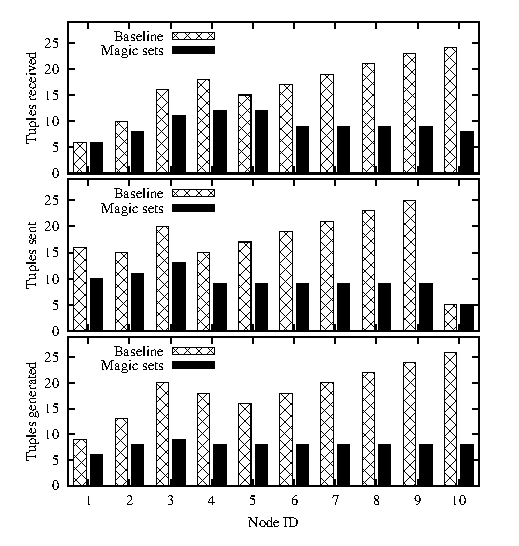
\includegraphics{figures/magicNumbers}
\ssp
\caption{For each node (node ID on $x$ axis), number of tuples received
  (top), sent (middle), and locally generated (bottom) on the $y$ axis.}
\label{ch:evita:fig:magicresults}
\end{figure*}

Figure~\ref{ch:evita:fig:magicresults}(a) shows the number of tuples that each
node receives from the network.  The magic-sets rewritten program causes no
more tuples to be received than the original, and for most nodes significantly
fewer when moving to nodes farther away from the clique.  That is because many
paths that are generated in the original program with destinations within the
clique other than node $node1$ are pruned early on and never transmitted all the
way to the far end.  Similarly, Figure~\ref{ch:evita:fig:magicresults}(b) shows
the number of tuples each node transmits.  Again, the magic-rewritten program
does a lot better.  The two programs have similar tuple transmit/receive
overheads for nodes represents the number of tuples a node sends out over the
network.  

The inclusion of the magic-sets rewrite reduces the number of sends in all but
one case ($node10$).  We note here that the edges from $node10$ to $node4$ are
directed.  As a result, $node10$ is the only node with no incoming links and is
therefore never burdened with network traffic other than its own.  As a result,
its transmit tuple overhead is unaffected, since it already sends out no
extraneous paths other than its own path to other nodes.  Finally, tuple
storage is impacted beneficially by magic sets everywhere
(Figure~\ref{ch:evita:fig:magicresults}(c)), since both \ol{path} tuples
received from the network, and those generated locally for local consumption
are pruned away by the rewrite.



